\section{Study Design}
\label{sec:study}

\subsection{Network and IBR plants}

The study uses the 37-bus network of \cite{gloverPSAD}: 37 buses, 42 lines, 14 transformers, 26
loads totalling 806~MW and 281~Mvar, seven synchronous generators plus a slack at bus 31, and a 100-MVA base. Three IBR
plants of 60, 45 and 45~MW are connected at their POIs, the 69-kV buses 21, 48 and 16
(Fig.~\ref{fig:network}). Each plant is modelled as in Fig.~\ref{fig:plant}: a 69/34.5-kV main
transformer, a collector feeder to the MV bus, a 34.5/0.69-kV padmount transformer and one
aggregate converter. Following \cite{dhungana2026}, the converter is rated at 1.1 times the
plant's active power and each transformer at 1.2 times the converter rating, with
$0.005 + j0.06$~pu on its own base. The converters inject their rated active power at unity
power factor in every state, the case in which they displace the most synchronous generation.
Adding the plants gives the 46-bus network on which ESCR and SDSCR
are evaluated; SCR and WSCR use the 37-bus network without them (Table~\ref{tab:conventions}).

\begin{figure}[!t]
\centering
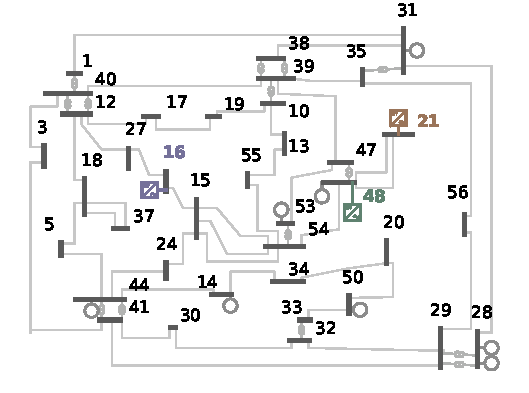
\includegraphics[width=\linewidth]{f1a_network}
\caption{The 37-bus network with the three IBR plants at buses 21, 48 and 16.}
\label{fig:network}
\end{figure}

\begin{figure}[!t]
\centering
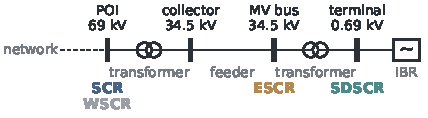
\includegraphics[width=0.85\linewidth]{f1b_plant}
\caption{Model of one IBR plant and the evaluation point of each metric: POI, MV bus and
converter terminal.}
\label{fig:plant}
\end{figure}

\subsection{Operating states}

Public hourly demand for the Swedish bidding zone SE3 in 2025 serves only as a scaling signal.
The 168-hour window with the largest load range, starting \NumWeekStart~UTC, scales
every load's active and reactive power by the hourly demand divided by the window mean. The load
scale ranges from \NumLoadScaleMin{} to \NumLoadScalePeak.

Generation is committed by one of two rules. Under the largest-first rule, the non-slack units
are committed in descending order of maximum output, each within its limits, until the remaining
demand is below the next unit's minimum output; the slack takes the rest. With every unit online,
all non-slack units run at a common fraction of their maximum output, not below their minimum,
and the slack takes the rest. The 37-bus network dispatches the full demand and the 46-bus
network the demand less the IBR plants' 150~MW, each with its own schedule. Under the largest-first
rule, between \NumUnitsFewestNoIBR{} and \NumUnitsMostNoIBR{} units are committed on the 37-bus
network and between \NumUnitsFewestIBR{} and \NumUnitsMostIBR{} on the 46-bus network. Each
state is a Newton--Raphson power flow with generator reactive limits and the case's automatic tap
controllers; the IBR transformers keep nominal taps.

\subsection{Branch outages}

Every line and transformer of the 37-bus network whose outage islands no bus and leaves both
networks solvable in all 168 hours is outaged in turn: \NumLinesOut{} of the \NumLinesAll{} lines
and \NumTransformersOut{} of the \NumTransformersAll{} transformers. The IBR plants' own transformers are not outaged,
since that would disconnect the plant. Commitment and dispatch are held at the intact schedule, so an outage changes only the topology. The pre-fault voltages then follow from the power flow. 
The \NumOutages{} outages fall into \NumCorridors{} corridors, since parallel branches count once
(lines 18--37, 21--48 and 15--54; transformers 12--40, 28--29, 38--39 and 41--44).

\subsection{Experiments and validation}

The metrics are evaluated on three sets of states, \NumStates{} in all: the intact week under the
largest-first rule, the same week under each branch outage, and the intact week with every unit
online.

To test the interaction-factor convention, ESCR is also computed on the first two sets with a
voltage-step factor in place of the impedance-based reference. An ideal voltage source with zero
active power at bus $i$ raises $|V_i|$ by a step of 0.5, 1 or 2\,\% in a power flow started
from the solved state, with taps frozen and the generators regulating their voltages. The factor
$\mathrm{MIIF}_{ji} = \Delta V_j/\Delta V_i$ then includes their response.

The fault calculation was checked against PowerWorld on the base case
and six other network configurations with generator, line or transformer changes, with fault currents agreeing within \NumPowerWorldMaxErrorPct\,\%.
